\Section{Deep Learning and Conditional Invertible Neural Networks}
\label{ch:deeplearning}

Deep Learning is a subdomain within Machine Learning focusing on the construction and training of deep neural networks. Such networks have been proven to be extremely successful in different, analytically unsolvable problems such as (but not restricted to) image classification tasks, regression tasks, image generation tasks, language translation and reinforcement learning.

In this chapter, a brief introduction to these networks and their properties with a focus on so-called normalizing flows and invertible neural networks is given.

\Subsection{Foundations of Deep Learning and Neural Networks}
\Subsubsection{The Universal Approximation Theorem}

The success of Neural Networks (NNs) lies in their potential of learning (almost) arbitrary models. This property of NNs can be expressed mathematically through the Universal Approximation Theorem which in words states a feed-forward network with linear output and at least one hidden layer with a finite number of nodes can approximate any real continuous function on a given closed and bounded subset to arbitrary precision \cite{DLiPR}.

However, the Universal Approximation Theorem does not state how the network should be constructed to achieve the desired precision. For this reason, the theorem has been proven for several network architectures; in case of ReLU-activated feed-forward networks the theorem can be written as the following \cite{UAC}:
\newtheorem{theorem}{Theorem}
\begin{theorem}
	For any real and continuous function $f : [0, 1]^{d_{in}} \rightarrow \mathbb{R}^{d_{out}}$ and every $\epsilon>0$ there is a ReLU-network $\mathcal{N}$ with the same input and output dimension $d_{in}$ and $d_{out}$ and a minimum hidden layer width $w_{min}$ for which
	\begin{equation*}
		\sup_{x\in[0, 1]^{d_{in}}}\Vert f(x)-f_\mathcal{N}(x)\Vert \leq \epsilon
	\end{equation*}
	and
	\begin{equation*}
		d_{in} + 1 \leq w_{min}(d_{in}, d_{out}) \leq d_{in} + d_{out}
	\end{equation*}
\end{theorem}
This theorem does not state anything about the exact depth (number of layers) the network needs to have, its speed of convergence and the optimization process it needs to undergo to achieve this arbitrary approximation. On the other hand, it is reassuring to have a mathematical guarantee for convergence for a given feed-forward network structure. For this reason, empiric studies are usually performed to look for a locally optimal solution for a given task.

In the following, a brief overview of the most common NN components is going to be given with special focus on the ones used for the construction of the cINN.

\Subsubsection{Fully-Connected Neural Networks}
The most elementary NNs perform affine transformations (consisting of a linear transformation represented by a weight matrix $W$ and a shift $b$) on a given input $x$ followed by the application of a non-linear function (called activation) $g$:

\begin{equation*}
	y = g(Wx+b)
\end{equation*}

Graphically, one such transformation is represented as a layer. For a fully-connected neural network, these transformations are called in succession, resulting in stacked layers of $n$ nonlinearities as shown in fig. \ref{fig:nn}. The resulting mapping

\begin{equation*}
	f(x, \theta) = g^n\left\{W^{n-1}g^{n-1}\left[ ... \left(W^2g^1(W^1x+b^1)+b^2\right)...\right]+b^{n-1}\right\}
\end{equation*}

is a universal approximator with the free parameters $\theta$ (containing all the matrices $W^i$ and the biases $b^i$) for the target output for $y$. Finding the optimal parameters $\theta$ is called training and the $\theta$ will be referred to as trainable parameters. The graphical representation of a neural network mapping is shown in fig. \ref{fig:nn}.

\tikzset{%
	every neuron/.style={
		circle,
		draw,
		minimum size=1cm
	},
	neuron missing/.style={
		draw=none, 
		scale=2.5,
		text height=0.333cm,
		execute at begin node=\color{black}$\vdots$
	},
}
\begin{figure}[h!]
	\centering
	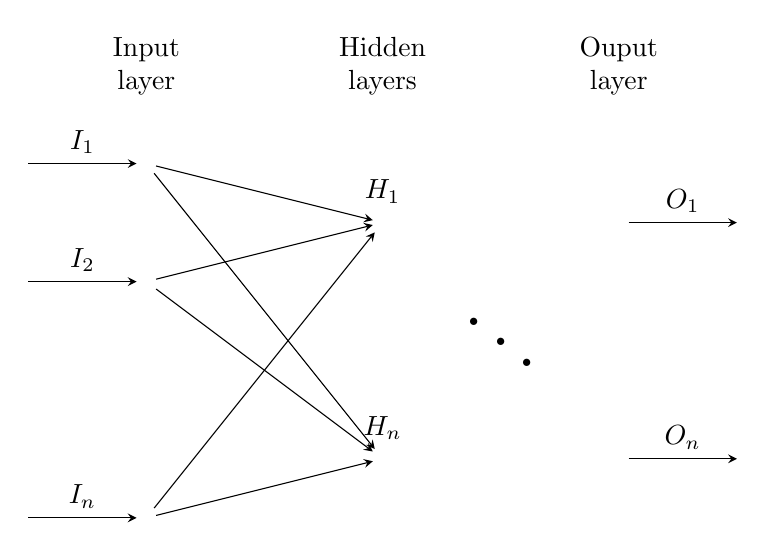
\begin{tikzpicture}[x=1.5cm, y=1.5cm, >=stealth]
		
		\foreach \m/\l [count=\y] in {1,2,missing,3}
		\node [every neuron/.try, neuron \m/.try] (input-\m) at (0,2.5-\y) {};
		
		\foreach \m [count=\y] in {1,missing,2}
		\node [every neuron/.try, neuron \m/.try ] (hidden-\m) at (2,2-\y) {};
		
		\foreach \m [count=\y] in {1,missing,2}
		\node [every neuron/.try, neuron \m/.try ] (output-\m) at (4,2-\y) {};
		
		\foreach \l [count=\i] in {1,2,n}
		\draw [<-] (input-\i) -- ++(-1,0)
		node [above, midway] {$I_\l$};
		
		\foreach \l [count=\i] in {1,n}
		\node [above] at (hidden-\i.north) {$H_\l$};
		
		\foreach \l [count=\i] in {1,n}
		\draw [->] (output-\i) -- ++(1,0)
		node [above, midway] {$O_\l$};
		
		\foreach \i in {1,...,3}
		\foreach \j in {1,...,2}
		\draw [->] (input-\i) -- (hidden-\j);
		
%		\foreach \i in {1,...,2}
%		\foreach \j in {1,...,2}
%		\draw [->] (hidden-\i) -- (output-\j);
%		\draw [->] (hidden-1) -- (output-1);
%		\draw [->] (hidden-2) -- (output-2);
		
		\foreach \l [count=\x from 0] in {Input\\ layer, Hidden\\ layers, Ouput\\ layer}
		\node [align=center, above] at (\x*2,2) {\l};
		
		\node [draw=none, scale=2.5, text height=0.333cm] at (3, 0) {$\ddots$};
		\node [draw=none, scale=2.5, text height=0.333cm] at (3, 1.25) {$\hdots$};
		\node [draw=none, scale=2.5, text height=0.333cm] at (3, -0.75) {$\hdots$};
		
	\end{tikzpicture}
	\caption{Schematic structure of a feed-forward NN. The nodes represent the variables for the hidden and output layers or the biases and the activations $g$ applied to the intermediate outputs for the hidden layers. Arrows represent the matrix $W$.}
	\label{fig:nn}
\end{figure}

Note that for the approximation to work arbitrary well, the structure of the network and training have to be correctly adjusted to the task to be solved.

\Subsubsection{Activation Functions}
It is essential for convergence to select the right activation function $g$. Historically, several candidate activation functions such as sigmoid, tanh, the rectified linear unit (ReLU) and its variants such as SeLU and leaky-ReLU have emerged. In this work ReLU will be used exclusively. An advantage of ReLU is the lack of saturation range compared to the sigmoid or the tanh activation functions, where gradients above or below a given value of $x$ become negligible, "paralysing" the training. Apart from that, ReLU has tractable derivatives and has proven to be an efficient activator empirically. It is defined as

\begin{equation*}
	\text{ReLU}(x) = \max \{0, x\}
\end{equation*}

where the maximum is taken element-wise over the vector components of $x$. Note that its derivative is not continuous and makes a jump at the origin from 0 to 1, which renders parameters 0 during training. On the other hand, this activation function has no scale, making it an excellent candidate for general approximation tasks. A graph of the most commonly used activation functions is shown in fig. \ref{fig:activations}.

\begin{figure}
	\centering
	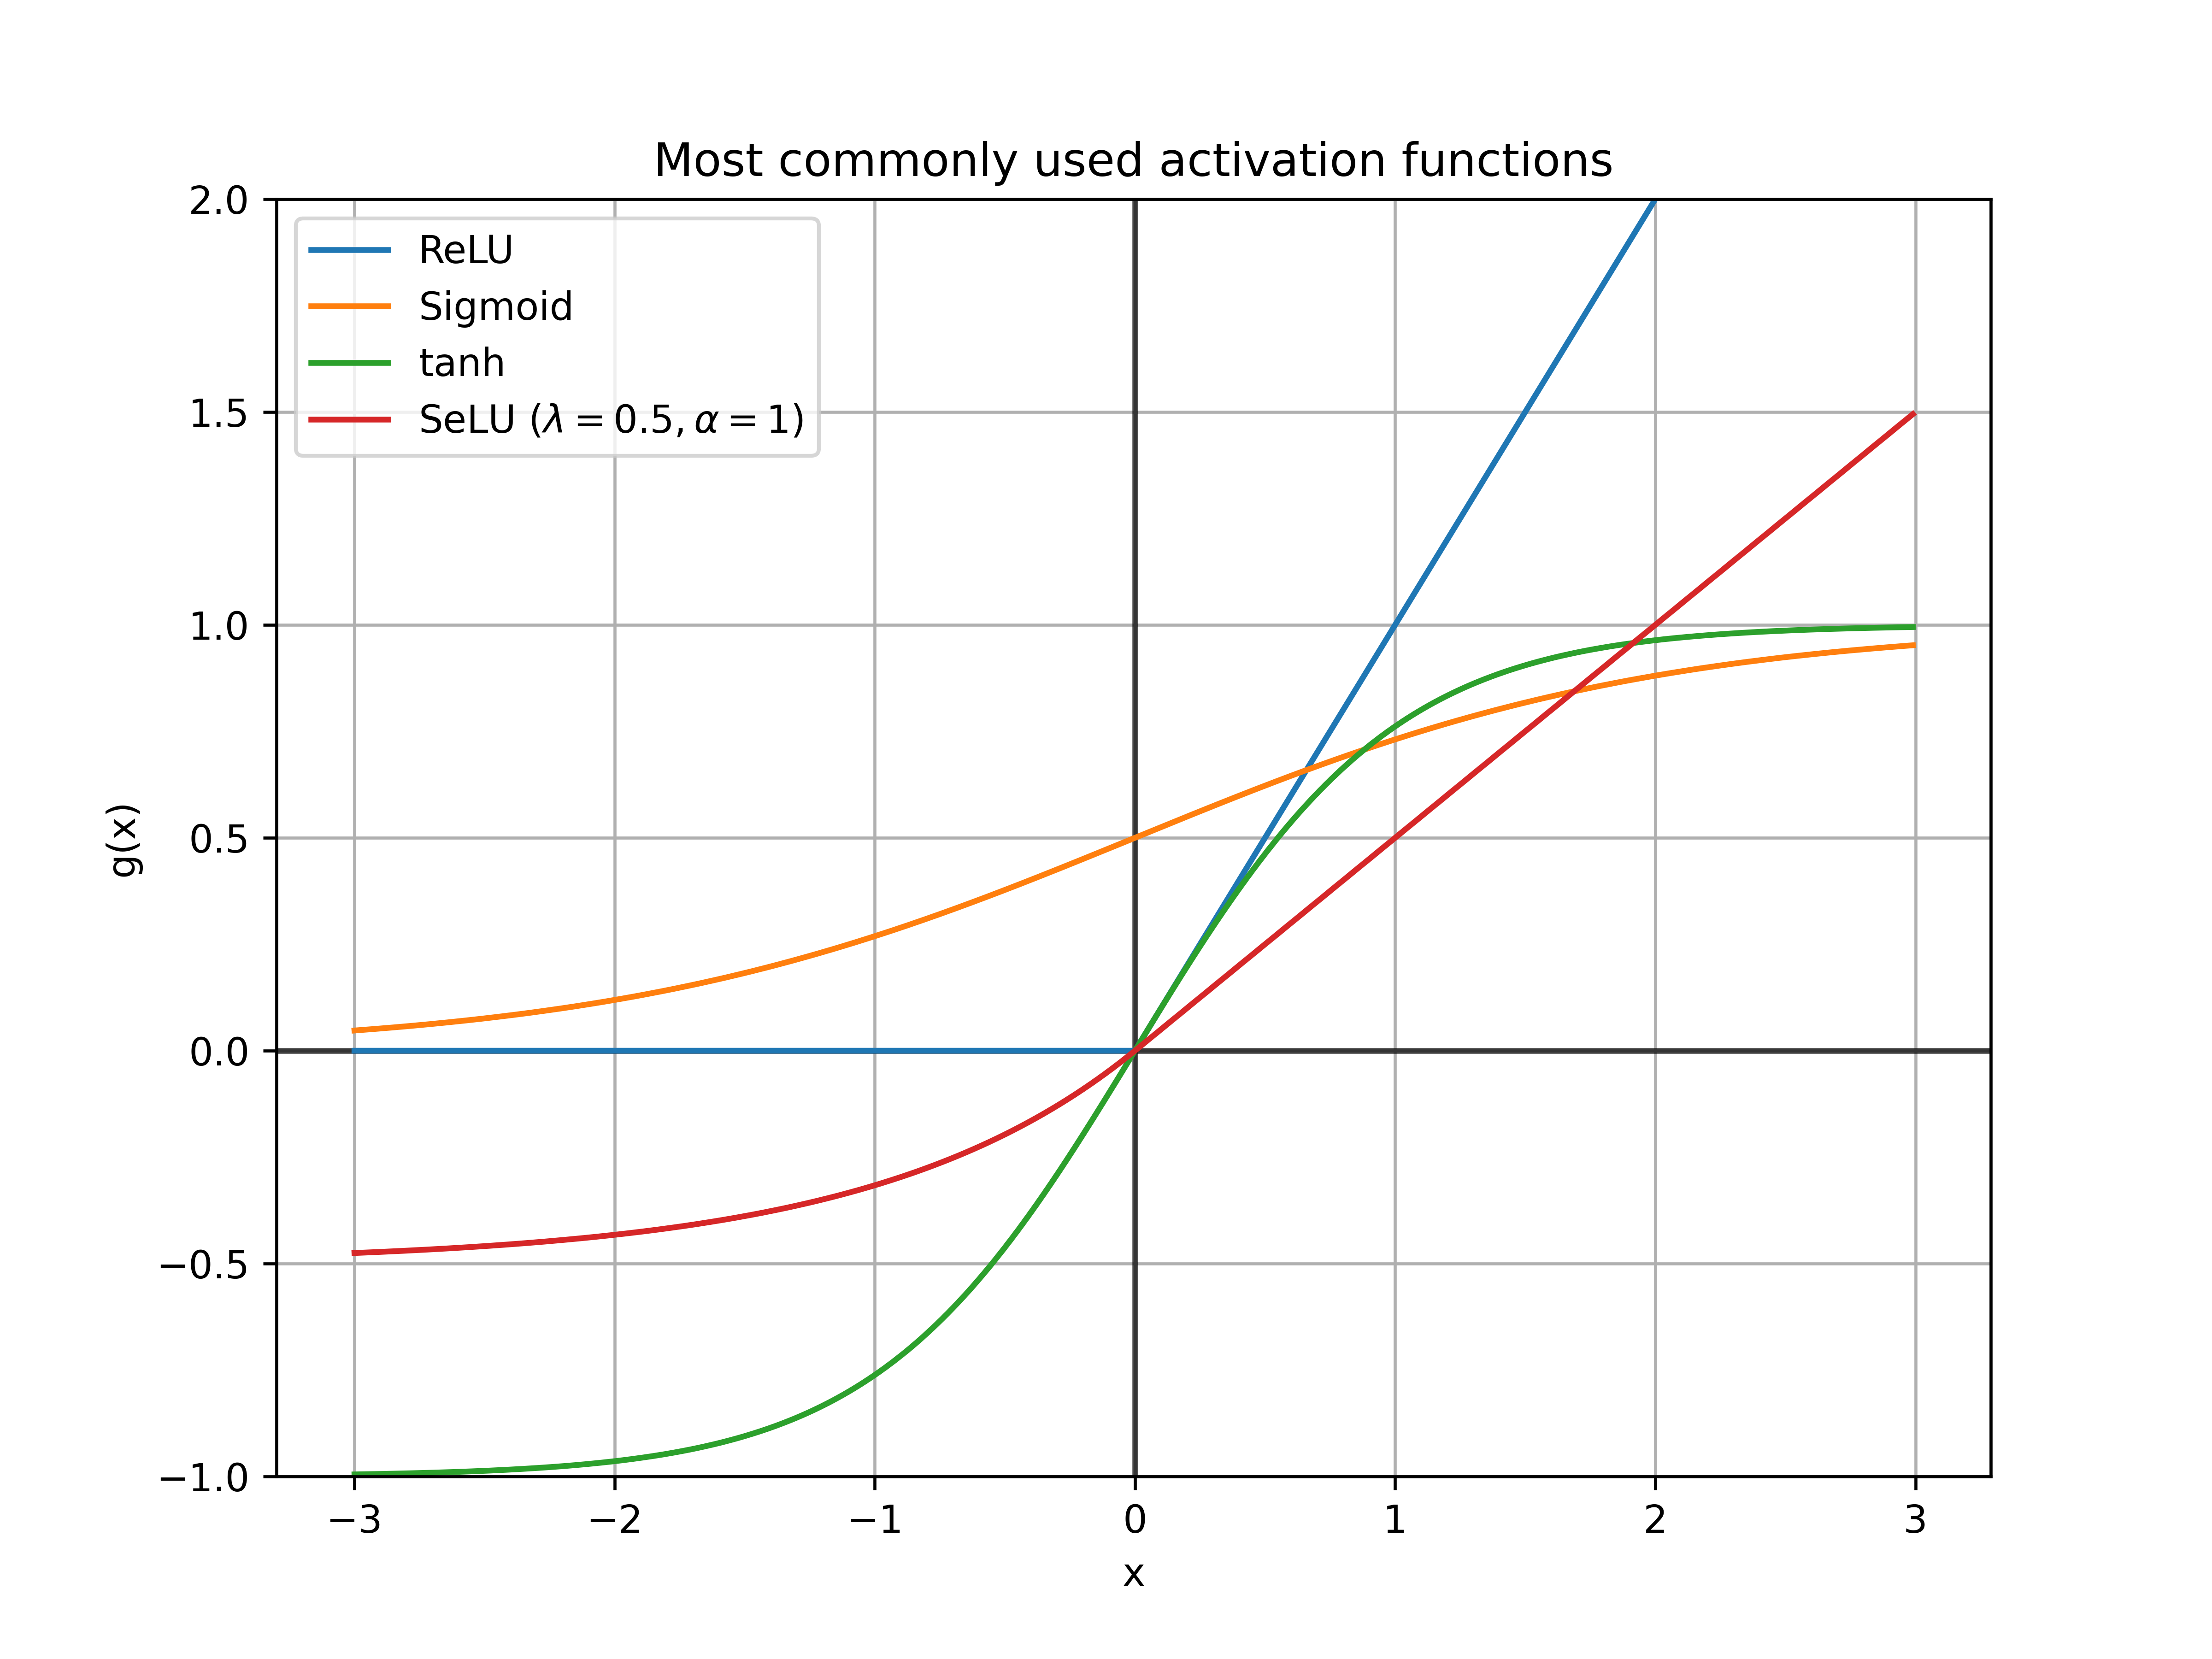
\includegraphics[width=0.7\linewidth]{figures/neural_networks/activations}
	\caption{Most commonly used activation functions. Note the plateaus of the sigmoid and tanh functions and for all $x$<0 for ReLU. Setting the gradient zero in case of ReLU for $x$<0 renders several parameters inactive during training; on the other hand, large positive parameters do not get stuck due to vanishing gradients and the function is scaleless.}
	\label{fig:activations}
\end{figure}

\Subsubsection{Objective Functions}

Having established the network structure, a measure of fit quality remains to be chosen. Such measures are called objective functions (error or loss functions) and used to govern the training by setting the gradients of the trainable parameters $\theta$.
Several loss functions have been established for each NN-specific task to be solved. The mean-squared-error (MSE) has been found useful for regression tasks due to its resemblance to the least-squared-error obtained from likelihood fits of normal distributed data. The so-called cross-entropy error function has been found performant for classification tasks due to the relation of the loss to information theory and the accessible probabilistic interpretation of the outputs following sigmoid activation. Both of these loss functions need target labels to compare the network outputs to. Training procedures where fixed labels guide the parameter estimation are called supervised learning.

Distribution fitting requires the loss function to compare samples from a probability distribution function to a target distribution. Since the discrete labels are replaced with continuous target distributions and none of the datapoints has a well-defined target these training procedures belong to the class of unsupervised learning. As the name suggests, the neural network does not obtain any additional feature representation of the data necessary for the optimization procedure. In layman's terms the network has to "figure out on its own" which input features are more important for the given task.

In this work, distribution fitting will be performed which is reflected by the choice of the loss function. The Kullback-Leibler divergence (also called relative entropy) is a measure of resemblance of $p_\text{x}(x; \theta)$ to $q_\text{x}(x)$, both defined over the random variable \text{x}, and belongs to the families of $f$-divergences defined as

\begin{equation*}
	D_f\left[q_\text{x}(x) \, \, || \, \, p_\text{x}(x; \theta)\right] = \mathbb{E}_{p_\text{x}(x; \theta)}\left[f\left(\frac{q_\text{x}(x)}{p_\text{x}(x; \theta)}\right)\right]
\end{equation*}

with the convex function $f(r) = r\log r$ \cite{Papamakarios_NF}. In its expanded form it can be written as

\begin{equation}
	\begin{aligned}
		\mathbb{KL}\left[q_\text{x}(x) \, \, || \, \, p_\text{x}(x; \theta)\right] &= \mathbb{E}_{q_\text{x}(x)}\left[\frac{\log q_\text{x}(x)}{\log p_x(x; \theta)}\right] \\&= \underbrace{- \mathbb{E}_{q_\text{x}(x)} \left[ \log p_\text{x}(x; \theta)\right]}_{\mathcal{L}(\theta)} + \underbrace{\mathbb{E}_{q_\text{x}(x)}\left[\log q_\text{x}(x)\right]}_{const}
	\end{aligned}
	\label{eq:KL-loss}
\end{equation}

and can be decomposed into a $\theta$-parameter dependent and a $\theta$-independent term\footnote{Note that the Kullback-Leibler divergence is not symmetric in its arguments and swapping $q$ and $p$ does not yield a similar decomposition due to the expectation value taken over the probability density function $p_\text{x}(x; \theta)$. Hence a distinction between the forward and the backward Kullback-Leibler divergence has to be made. In to following, the forward KL-divergence (introduced above) will be used exclusively.}. The KL-divergence has a global minimum of value 0 where both distributions are identical. With this expression, one can approximate an unknown posterior distribution $p(x | y)$ using a model function $p_\theta(x | y)$ (both conditioned on a random variable $y$) by taking the parameter-dependent term $\mathcal{L}(\theta)$ as a basis for the loss function.

Objective functions "guide" only the training, but are not a measure about the quality of the predictions per se. It can occur in terms of the weights, that a given feature of one or several inputs enjoys a higher-than-optimal weight at the cost of generalization (overfitting and overtraining). For this reason, the entries of the weight matrix during gradient descent are penalized with an additional $L^2$ regularization term

\begin{equation}
	L'(\theta) = L(\theta) + \alpha \, ||\theta|| _2^2
\end{equation}

where $\alpha$ is a fixed regularization parameter.

What is missing from a complete training is data the network is trained with respect to and the optimizer looking for an optimum of the loss function.

%With this choice of the loss, one can potentially generate samples from the true posterior distribution at the global optimum of the KL-divergence. In the following, a likelihood-free solution to the posterior inference problem using conditional invertible neural networks will be discussed.

\Subsubsection{Training and Loss Optimization}

The optimization is data-driven. The dataset is split up to two disjoint datasets: a training and a test set. For every iteration a number of samples from the training set are evaluated through the network from which the current network performance can be evaluated. Ideally, finding a local optimum of a one-dimensional function requires a closed form of the function itself with respect to its parameters. Unfortunately, this is usually not the case due to the high-dimensional and nonlinear nature of the optimization problem. For this reason, the weight matrices are adjusted for every node through backpropagation: the gradients for each hyperparameter are calculated from the previous layer and the parameters are updated through gradient descent along the negative of the parameter gradient moving slowing to a locally optimal value. For a simple case, it can be intuitively written with a positive learning rate $\eta$ as

\begin{equation}
	\theta^t = \theta^{t-1}-\eta\left[\frac{\partial \mathcal{L}}{\partial\theta}\right]^{t-1}
	\label{eq:optimization}
\end{equation}

Note that the learning rate is a decisive parameter in the update process; while a too small value of $\eta$ does not improve the loss significantly, a large $\eta$ on the other hand cannot achieve the desired convergence. To speed up the optimization process, this simple idea has been improved further upon and several competing optimizers have emerged. In this work, the quasi-standard Adam optimizer \cite{Adam_paper} has been used. It uses a sophisticated self-tuning learning rate optimization (taking the "momentum of convergence" into consideration) and several, empirically useful parameters to optimize the convergence. The algorithm can be summarized as the following:

\begin{equation*}
	\begin{cases}
			\theta^{t+1} &= \theta^t - \eta \cdot \frac{\hat{m}^t}{\sqrt{\hat{v}^t}+\epsilon}\\
			g^t &=\nabla_\theta f^t (\theta^{t-1})\\
			m^t&=\beta_1 \cdot m^{t-1} + (1-\beta_1) \cdot g^t \\
			v^t&=\beta_2 \cdot v^{t-1} + (1-\beta_2) \cdot g^t \\
			\hat{m}^t&=\frac{m^t}{1-\beta^t_1}\\
			\hat{v}^t&=\frac{v^t}{1-\beta^t_2}
	\end{cases}
\end{equation*}

Note that while Adam evaluates the next step using multiple measures in a sophisticated manner, in its core and using the right parameters the same gradient descent from eq. \ref{eq:optimization} can be found. It has been found experimentally that the parameters $\beta_1 = 0.9$ and $\beta_2 = 0.999$ are suitable choices for general tasks.

In order to further improve the optimization, the updates are evaluated for a fixed number of samples (batches) which introduces a stochastic nature to it averaging the gradient for the selected samples. The main advantage of stochastic gradient descent is the consecutive updates towards a more general optimum and avoiding getting stuck at local optima due to strongly varying gradients evaluated from the dataset.
Once the whole training dataset has been used up, an epoch has reached its end and the process starts anew with a shuffled training dataset. After several epochs, the procedure converges.
In order to monitor the network performance and its generalization capabilities, the test set is used. For this, the loss can be evaluated for these "unseen" datasamples, which can show signs of anomalies during training. Should for example the test loss rise while the training loss decreases, one can be certain that overtraining has had occurred.

\Subsection{Conditional Invertible Neural Networks}

Conditional Invertible Neural Networks have been found performant in machine learning tasks such as image colouring and guided image generation with style transfer \cite{cINN_im_gen}, parton shower generations and detector effect simulation \cite{Bellagente_2020}, stellar parameter determination \cite{Ksoll_2020} and cosmic ray source property inference \cite{Bister_2022}.

Most neural network setups tackle the challenge of posterior inference where the probability distribution 

\begin{equation*}
	p(x | y) = \frac{p(y | x) p(x)}{p(y)}
\end{equation*}

in Bayes' Theorem cannot be evaluated analytically. Most of these models are constructed in a one-directional way and do not preserve probability during inference. For this reason, even for (potentially) invertible problems, the model inverse is ill-defined. To avoid this, the network architecture has to be adjusted to satisfy the requirements of invertibility.

\Subsubsection{General INN Architecture}

To ensure invertibility the network input and output dimensions have to match to fulfil bijection. General invertible neural networks map the inputs $x$ to their targets $y$ while encoding some information regarding $x$ in the latent variables $z$. These variables are assumed to follow a fixed distribution which is also represented in the loss function. Usually these distributions are chosen to be a multivariate normal distribution, as they are unbiased and easy to sample from, the latter being crucial for obtaining the posterior distributions $p(x | y)$. Indeed, it can be shown that upon perfect convergence sampling from the latent space and picking an $y$ network inference yields the true posteriors $p(x | y)$ for any $y$ \cite{INN_Ardizzone}.

\begin{figure}[h!]
	\centering
	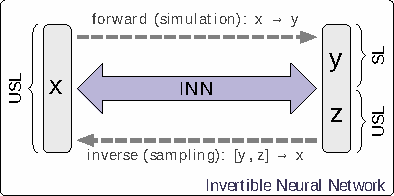
\includegraphics[width=0.6\linewidth]{figures/neural_networks/inns.pdf}
	\caption{General INN structure. Uniquely to these structures\protect\footnotemark, the network can be trained in both directions with a supervised loss (SL) term for the target labels $y$ and an unsupervised loss term (USL) for the latents $z$ and inputs $x$. \cite{INN_Ardizzone}}
	\label{fig:inn}
\end{figure}

\footnotetext{but not for cINNs}

A conceptual disadvantage arises from the conditions being included in the network outputs. Assuming the dimensionality of $x$ and $y$ are wide apart from each other zero-padding or several noise-extending techniques are necessary to construct the network potentially introducing unnecessary redundancies. This can be fixed by removing the conditions $y$ from the output and by using them as an additional input for the network and by setting the dimension of the latent space distribution to match that of the inputs $x$. With this approach, the conditions can also be pre-processed by applying a -- either pre- or jointly with the network trained -- network (a conditioning or summary network) \cite{BayesFlow}. Such setups enable processing of highly correlated or feature-rich data at the cost of potential overfitting \cite{Ksoll_2020}. A sketch of the resulting network -- the conditional invertible neural network (cINN) -- structure is shown in fig. \ref{fig:cINN_archicture}.

\begin{figure}[h!]
	\centering
	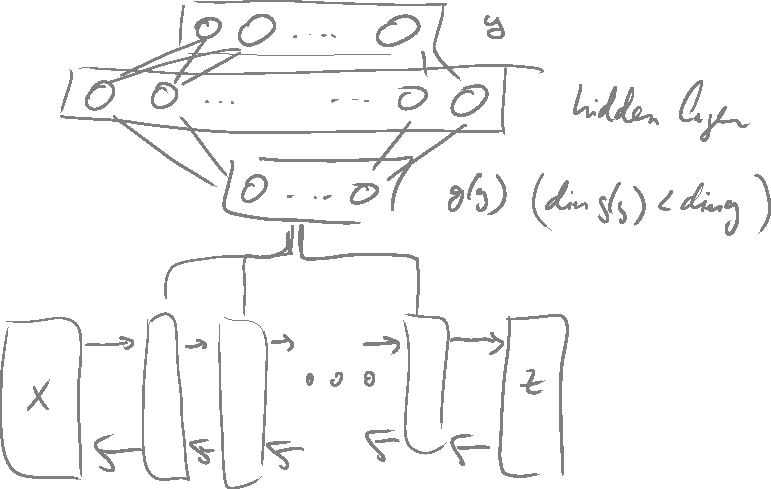
\includegraphics[width=0.4\linewidth]{figures/neural_networks/SN-cINN.pdf}
	\caption{\textcolor{red}{A sketch of the network setup with a summary network}}
	\label{fig:cINN_archicture}
\end{figure}

By constructing an invertible structure, the challenge of exact posterior inference remains with the added difficulty of mapping the inputs to the latent space distribution (LSD) in a meaningful (invertible and information conserving) way. To tackle this challenge, normalizing flows (NF) have to be applied.

\Subsubsection{Normalizing Flows}

The main idea of NFs is to construct an invertible transformation $T$ which maps a probability distribution $p$ to a target probability distribution $q$ in an invertible way. Hence, both $T$ and its inverse $T^{-1}$ have to be invertible and differentiable to preserve the probability flow. Such mappings are called diffeormophisms; note that a composition of diffeomorphisms

\begin{equation*}
	T' = T_1 \circ T_2 \circ ... \circ T_N
\end{equation*}

yields a diffeomorphism too.

In a historic sense a whitening transformation can be already viewed as a normalizing flow the target distribution being a (multivariate) normal distribution. In more general and complicated cases however, the transformation $T$ cannot be easily constructed by hand. As the transformation is applied to samples of the distribution $p$, the flow has to normalize the distribution internally.

Assume we would like to express the probability $p(x)$ using the target distribution. For this, a straightforward coordinate transformation involving the Jacobian from the source to the target space can be used:

\begin{equation*}
	p(x) = p(z) \left| \det J_T \right| = p(z) \left| \frac{\partial x}{\partial z} \right|
\end{equation*}

The backward transformation can be written using the inverse of $T$ and its determinant

\begin{equation*}
	p(z) = p(x) \left| \det J_{T^{-1}} \right| = p(x) \left| \frac{\partial z}{\partial x} \right|
\end{equation*}

Here we can directly observe the explicit reason why $T$ has to be diffeomorphism. A graphical representation of a normalizing flow for two-dimensional distributions can be seen in fig. \ref{fig:NF_example}.

\begin{figure}[h!]
	\centering
	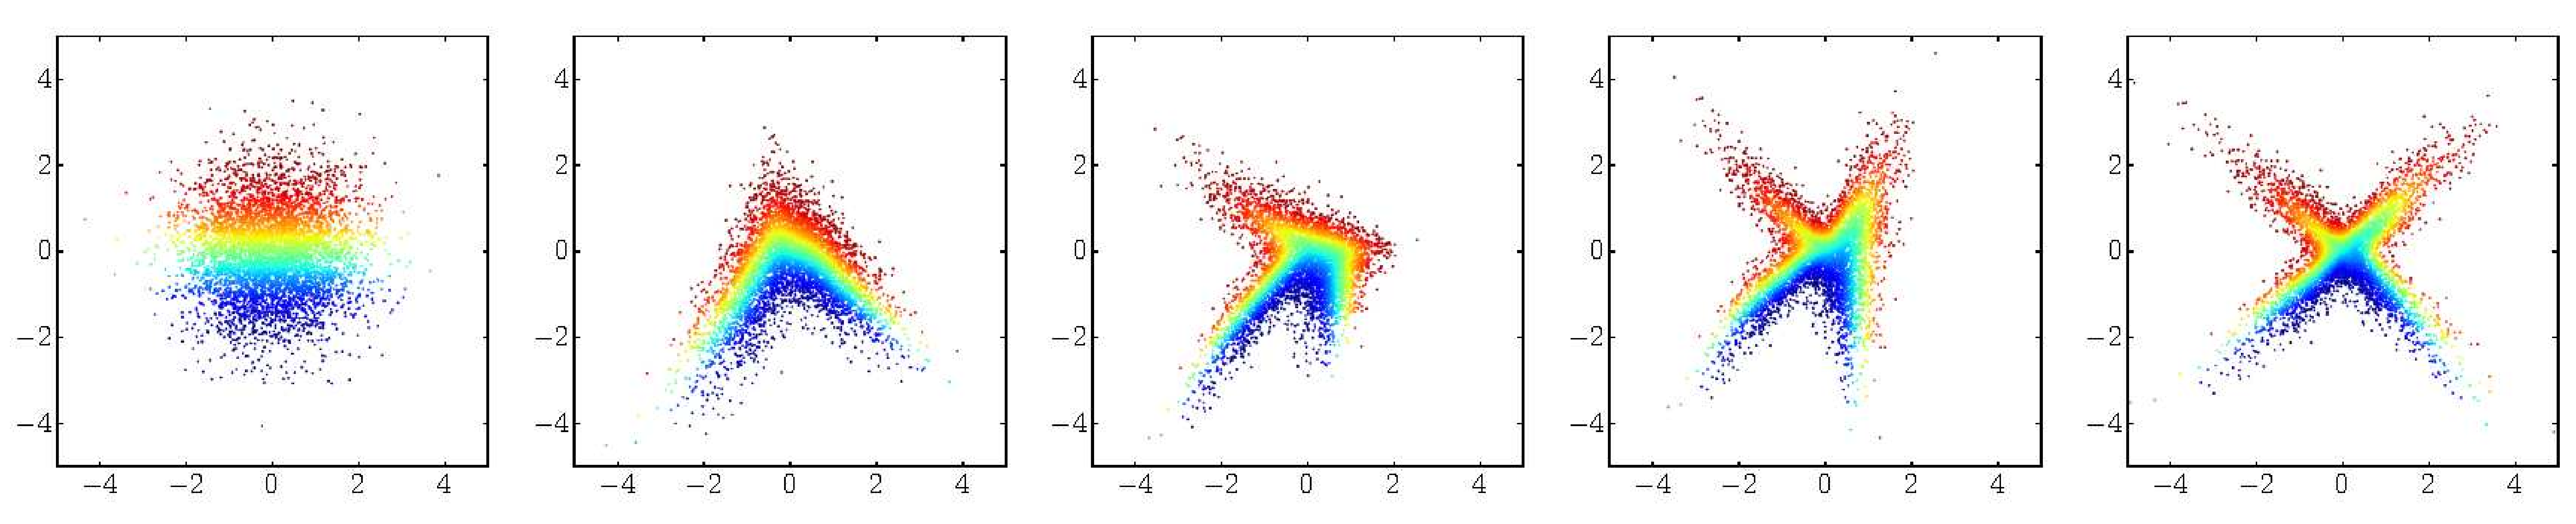
\includegraphics[width=\textwidth]{figures/neural_networks/flow}
	\caption{Example of a normalizing flow transforming a normal distribution to a star-shaped one in 4 steps. Note that the subsequent steps are also done with diffeomorphisms while the resulting transformation still remains a diffeomorphism. \cite{Papamakarios_NF}}
	\label{fig:NF_example}
\end{figure}

cINNs use neural networks to learn the mapping $T$. In the following, the construction of the diffeomorphic transformation will be discussed in detail.

\Subsubsection{Affine Coupling Blocks}

To represent the transformation $T$ Affine Coupling Blocks (ACB) can be utilized. In this work, exclusively the Generative Flow (GLOW) coupling block \cite{glow_paper} will be used. The GLOW block follows a design similar to the RealNVP block from \cite{RealNVP}. These blocks in practice need to fulfil at least two conditions: first, they have to invertible and second, the Jacobian of the mapping it represents has to be numerically tractable, especially its determinant. The GLOW block fulfils both of these conditions. In order to do so, it first splits up its input $u = [u_1, u_2]$ in two equal parts, on which a scaling $s_i(\cdot)$ and a translation $t_i(\cdot)$ using arbitrary, non-invertible functions are applied. The resulting transformation reads

\begin{equation}
	\left\{\begin{aligned}
		v_1 &= u_1 \odot \exp(s_2(u_2)) + t_2(u_2) \\
		v_2 &= u_2 \odot \exp(s_1(v_1)) + t_1(v_1)
	\end{aligned}\right.
	\label{eq:glow_transformation}
\end{equation}

where $\odot$ denotes the element-wise (Hadamard) product. Note that although the functions $s_i(\cdot)$ and $t_i(\cdot)$ are not necessary invertible themselves and can be approximated thanks to the Universal Approximation Theorem with neural networks, the transformation in eq. \ref{eq:glow_transformation} is invertible, as $u_1$ and $u_2$ can be expressed with $v_1$ and $v_2$:

\begin{equation*}
	\left\{\begin{aligned}
		u_1 &= (v_2 - t_1(v_1)) \odot \exp(-s_1(v_1)) \\
		u_2 &= (v_1 - t_2(u_2)) \odot \exp(-s_2(u_2)) 
	\end{aligned}\right.
\end{equation*}

At this point, the exponential functions may seem arbitrary. Looking at the Jacobian

\begin{equation*}
	\frac{\partial (v_1, v_2)}{\partial(u_1, u_2)} = \left(\begin{matrix}
		\exp(s_2(u_2)) & \frac{\partial v_1}{\partial u_2} \\
		0             & \exp(s_1(v_1))
	\end{matrix}\right)
\end{equation*}

and its determinant

\begin{equation*}
	\left|\frac{\partial (v_1, v_2)}{\partial (u_1, u_2)} \right| = \exp \left(\sum_j s^j_2(u_2) + s^j_2(v_1) \right)
\end{equation*}

it can be seen that they keep the determinant is nonzero independently of the behaviour of the scaling transformations $s_i(\cdot)$. It becomes also clear from the determinant, that even for high-dimensional input and output vectors $u$, $v$ the determinant is computationally cheap to evaluate.

Due to their mutual dependence on each other the expressions in eq. \ref{eq:glow_transformation} are not evaluated directly in practice and the transformation is split up in two intermediate steps. First, a term with

\begin{equation*}
	f_1(u_1, u_2) = (v_1, u_2) = \begin{cases}
		u_1 \odot \exp(s_2(u_2)) + t_2(u_2) \\
		u_2
	\end{cases}
\end{equation*}

is evaluated followed by

\begin{equation*}
	f_2(v_1, u_2) = (v_1, v_2) = \begin{cases}
		v_1 \\
		 u_2 \odot \exp(s_1(v_1)) + t_1(v_1)
	\end{cases}
\end{equation*}

It is easy to check, that the composed transformation $f = f_2 \circ f_1$ has the same Jacobian (and hence the same determinant) as the one in eq. \ref{eq:glow_transformation}. This step-wise evaluation can be visualized in a flow chart, as shown in fig. \ref{fig:glow}.

\begin{figure}[h!]
	\centering
	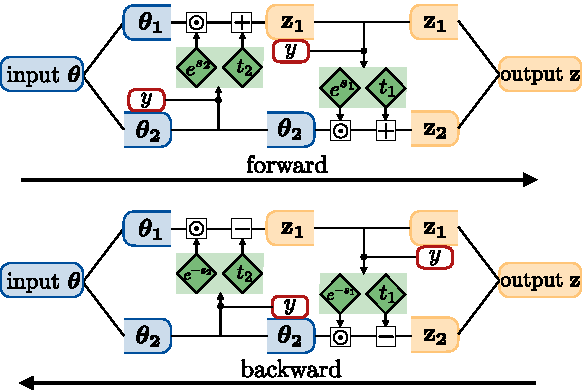
\includegraphics[width=\linewidth]{figures/neural_networks/glow.pdf}
	\caption{The forward and the backward pass of the GLOW block. Note that per construction, the sub-networks do not have to invertible themselves, and the block can be evaluated in both directions. The conditions node $c$ is used as an additional input for each sub-network. \cite{Ksoll_2020} \textcolor{red}{replace with Bister et al. sketch?}}
	\label{fig:glow}
\end{figure}

Note that the exponential functions in eq. \ref{eq:glow_transformation} can potentially produce extreme values which can lead to numerical instabilities during optimization. For this reason, additional soft-clamping is introduced, and an additional scale function with a fixed clamping coefficient $\alpha$ is applied to the scale coefficients $s_i(\cdot)$:

\begin{equation*}
	s' = \frac{2\alpha}{\pi} \arctan\left(\frac{s}{\alpha}\right)
\end{equation*}

For $\lim\limits_{s\rightarrow\pm\infty} s' = \alpha$, while $s' \approx s$ if $s$ is of the same order of magnitude as $\alpha$. This naturally dampens the gradients from one block to the other meaning $\alpha$ has to be carefully chosen to avoid information loss between the consecutive blocks. For most analyses clamping coefficients of $\alpha \approx 1.9$ suffices.

With the construction of the normalizing flow with the GLOW block and the subnetworks representing the scaling $s_i(\cdot)$ and transitions $t_i(\cdot)$, the setting of the loss function using the Kullback-Leibler divergence remains to construct the whole cINN.

\Subsubsection{The Kullback-Leibler Divergence as a Loss Function}

Our goal is to approximate the real posterior distribution of a physics parameter $x$ under the observation $y$, i.e. we would like to write:

\begin{equation*}
	p(x | y) \approx p_\theta(x | y)
\end{equation*}

With the Kullback-Leibler divergence from eq. \ref{eq:KL-loss}, this can be formalized with $q(x) = p(x | y)$ and $p(x; \theta) = p_\theta(x | y)$ as

\begin{equation*}
	\mathbb{KL}\left[p(x | y) || p_\theta(x | y) \right] = - \mathbb{E}_{p(x | y)} \left[ \log p_\theta(x | y)\right] + const.
\end{equation*}

This form of the KL-divergence can be understood in terms of likelihoods as finding the optimal parameters which maximize the likelihood is asymptotically equivalent to finding the distribution which has minimal distance to the real distribution in terms of the KL-divergence \cite{Bishop_book}. This expression can now be rewritten using the Jacobian and the known and fixed latent space distribution as

\begin{equation*}
	\begin{aligned}
		\mathbb{KL}\left[p(x | y) || p_\theta(x | y) \right] &= - \mathbb{E}_{p(x | y)}\left(\log p(z) \left|\det\frac{\partial z}{\partial x}\right|\right) + const. \\
		&= - \mathbb{E}_{p(x | y)}\left(\log p(z)  + \log \left|\det\frac{\partial z}{\partial x}\right|\right) + const.
	\end{aligned}
\end{equation*}

where $z = f(x, y, \theta)$ is the output of the network in the latent space. At this point we can fix the distribution $p(z)$ to be a multivariate Gaussian of mean 0 and standard deviation 1. Writing

\begin{equation*}
	p(z) \propto \mathcal{N}(z; \mu = 0, \Sigma=\mathbb{1}) \propto \exp\left(-\frac{z^2}{2}\right)
\end{equation*}

the resulting loss function becomes

\begin{equation*}
	\mathcal{L}(\theta) = \frac{1}{M} \sum_{m=1}^{M} \frac{f(x_m; \theta)^2}{2} - \log\left|\det\frac{\partial f(x_m; \theta)}{\partial x}\right|
\end{equation*}

for all inputs $x_m$ of batch $m$ to train the network with respect to.

\Subsubsection{Posterior Inference}
After training, the network should be capable of inferring the true posterior distribution. For this, a condition has to be fixed first. Then, one can select samples from the latent space distribution (as its shape has been fixed by the loss function) and invert the network to obtain the samples from the posterior distribution.
At first glance there is no guarantee from the loss and from the architecture only that it is meaningful to map the datapoints to a more or less arbitrary function, from which independently drawn samples can be used for posterior inference. However, it can be shown that the latent output distribution is statistically independent on the training data at the global optimum, and the latent output distribution is the same for any fixed condition \cite{BayesFlow}. This motivates the rightfulness of the sampling from the latent space.

